\documentclass[12pt]{article}

\usepackage[utf8]{inputenc}
\usepackage[brazil]{babel}
\usepackage[a4paper,left=3cm, right=2cm,top=2.5cm, bottom=2.5cm]{geometry}
\usepackage{amsmath}
\usepackage{graphicx}
\usepackage{float}
\usepackage{multirow}
\usepackage{authblk}
\usepackage{fancyhdr}
\usepackage{xcolor}
\usepackage{cite}


\title{\textbf{ENG1456 - Lógica Fuzzy - Trabalho 1}}
\author{\textbf{Aluno: Matheus Carneiro Nogueira - 1810764}}
\affil{}
\author{\textbf{Professora: Ricardo Tanscheit}}
\affil{}
\pagestyle{fancy}
\fancyhf{}
\lhead{{\small \textcolor{gray}{PUC-Rio ENG1456}}}
\renewcommand{\headrulewidth}{0pt}
\date{}
\renewcommand{\footrulewidth}{0pt}
\fancyfoot[C]{\thepage}

\begin{document}
	\maketitle
	\tableofcontents
	
	
	\begin{abstract}
		Este documento consiste no relatório do trabalho 1 do módulo de Lógica Fuzzy da disciplina ENG1456 da PUC-Rio. O trabalho consiste na construção de um sistema de inferência fuzzy para a previsão de um passo a frente de uma série temporal. Para tal, será utilizado o programa \textit{Fuzzy Rules}.
	\end{abstract}
	
	
\section{Parte 1 - Fuzzy Rules}

Com o intuito de realizar a previsão de um passo a frente da série temporal, foram testados diversos tamanhos de janela, número de conjuntos fuzzy e tipos de operações de interseção dos antecedentes, implicação e defuzzificação. Como os testes foram numerosos, aqui está exibido apenas o resultado da melhor configuração encontrada. Além disso, vale comentar que foi separada 80\% da série para treino, enquanto 20\% final foi separado para testes.

A tabela abaixo exibe os resultados de algumas das configurações testadas.

\begin{table}[H]
	\centering
	\begin{tabular}{|l|l|l|l|l|l|l|}
		\hline
		Num\_Conj & Janela & Intersec & Implicação & Defuzz  & Diff treino & Diff teste \\ \hline
		5         & 10     & min      & prod       & alt lim & 1.05        & 12.59      \\ \hline
		5         & 5      & prod     & prod       & alt lim & 1.49        & 1.70       \\ \hline
		5         & 15     & min      & min        & alt lim & 0.94        & 14.33      \\ \hline
		5         & 8      & min      & prod       & alt lim & 1.20        & 8.60       \\ \hline
		6         & 5      & prod     & prod       & alt lim & 1.31        & 2.00       \\ \hline
		6         & 7      & prod     & min        & alt lim & 1.04        & 3.59       \\ \hline
		6         & 10     & min      & min        & alt lim & 0.83        & 8.29       \\ \hline
		3         & 5      & min      & prod       & alt lim & 2.08        & 2.12       \\ \hline
	\end{tabular}
\end{table}

A fim de escolher a melhor configuração, avaliaremos o menor erro percentual de teste, isto é, \textit{Diff teste}. Dito isso, a melhor configuração é:
\begin{table}[H]
	\centering
	\begin{tabular}{|l|l|l|l|l|l|l|}
		\hline
		Num\_Conj & Janela & Intersec & Implicação & Defuzz  & Diff treino & Diff teste \\ \hline
		5         & 5      & prod     & prod       & alt lim & 1.49        & 1.70       \\ \hline
	\end{tabular}
\end{table}

Embora o erro de $1.7$ não seja pequeno, será escolhida essa configuração, haja vista a quantidade de parâmetros testadas. Vale notar que, em alguns casos, o erro do treino foi menor para outras configurações quando comparadas com essa. Note que, na maior parte desses casos, o tamanho da janela utilizada foi maior do que o tamanho da janela da configuração escolhida. Uma janela grande demais pode gerar um erro pequeno no treino ao mesmo tempo que gera um erro grande no teste, o que indica o problema de overfitting.

A figura abaixo exibe a interface do \textit{Fuzzy Rules} para as configurações selecionadas.
\begin{figure}[H]
	\centering
	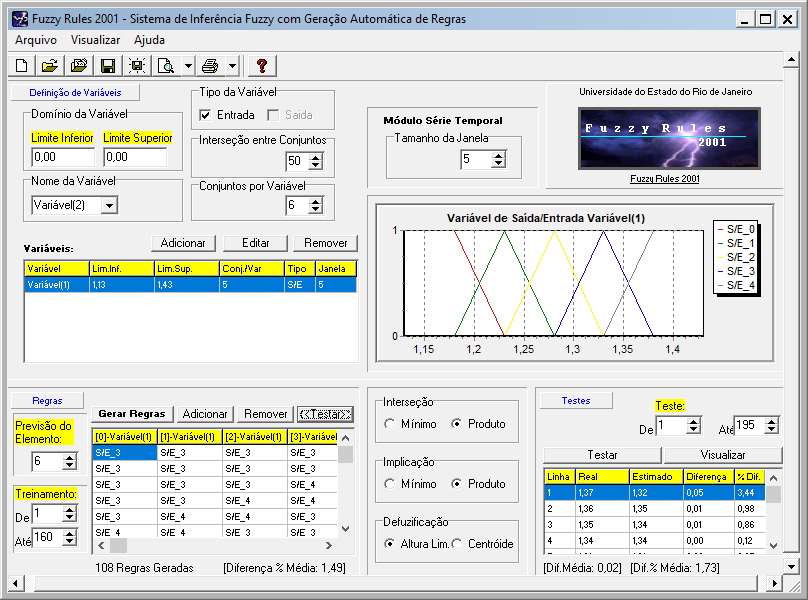
\includegraphics[width=0.7\linewidth]{Imagens/resultadoTeste_TUDO}
	\caption{Interface para configuração selecionada}
	\label{fig:resultadotestetudo}
\end{figure}



\section{Parte 2 - Extração Manual de Regras}
Tomando por base a melhor configuração obtida na seção 1 , foi realizado um passo a passo manual do procedimento de extração de regras para os dez primeiros dados do trecho da série especificado para a minha matrícula.

O passo a passo esquemático para a geração de regras consiste em:
\begin{enumerate}
	\item Definir tamanho da janela $\to$ 5
	\item Determinar o horizonte de previsão $\to$ 1
	\item Para cada regra, executar:
	\begin{enumerate}
		\item determinar o grau de pertinência dos valores da série dentro da janela e do horizonte
		\item atribuir, a cada variável, o conjunto de maior grau
		\item obter uma regra para cada par de entrada e saída
		\item Bônus:calcular o grau $D(R)$ para desfazer possíveis conflitos 
	\end{enumerate}
\end{enumerate} 

Como o enunciado solicita a extração para os 10 primeiros dados, 6 vezes pois, na sexta vez, usaremos o dado $x_{11}$ que já está além dos 10 primeiros dados pedidos. Vale lembrar que os 5 primeiros termos, referentes à janela, são os antecedentes e o sexto termo é o consequente. Além disso, os valores dos graus de pertinência foram tirados da análise do gráfico do \textit{Fuzzy Rules}.

\textbf{De $x_1$ até $x_6$}

\begin{align*}
	x_1=1.31=\begin{cases}
		SE_3=0.55\\SE_1=0.45
	\end{cases}\\
	x_2=1.34=\begin{cases}
		SE_3=0.70\\SE_4=0.30
	\end{cases}\\
	x_3=1.31=\begin{cases}
		SE_3=0.55\\SE_1=0.45
	\end{cases}\\
	x_4=1.31=\begin{cases}
		SE_3=0.55\\SE_1=0.45
	\end{cases}\\
	x_5=1.34=\begin{cases}
		SE_3=0.70\\SE_4=0.30
	\end{cases}\\
	x_6=1.37=\begin{cases}
		SE_3=0.20\\SE_4=0.80
	\end{cases}
\end{align*}

Atribuindo o maior grau de pertinência.
\begin{align*}
	x_1=1.31=\begin{cases}
		SE_3=0.55
	\end{cases}\\
	x_2=1.34=\begin{cases}
		SE_3=0.70
	\end{cases}\\
	x_3=1.31=\begin{cases}
		SE_3=0.55
	\end{cases}\\
	x_4=1.31=\begin{cases}
		SE_3=0.55
	\end{cases}\\
	x_5=1.34=\begin{cases}
		SE_3=0.70
	\end{cases}\\
	x_6=1.37=\begin{cases}
		SE_4=0.80
	\end{cases}
\end{align*}

Criando a regra e calculando o grau $D(R)$.
\begin{itemize}
	\item Se $x_1=SE_3$ e $x_2=SE_3$ e $x_3=SE_3$ e $x_4=SE_3$ e $x_5=SE_3$, então $x_6=SE_4$.
	\item $D(R)=0.55\cdot0.70\cdot0.55\cdot0.55\cdot0.70\cdot0.80=0.065$
\end{itemize}

\textbf{De $x_2$ até $x_7$}

\begin{align*}
	x_2=1.34=\begin{cases}
		SE_3=0.70\\SE_4=0.30
	\end{cases}\\
	x_3=1.31=\begin{cases}
		SE_3=0.55\\SE_1=0.45
	\end{cases}\\
	x_4=1.31=\begin{cases}
		SE_3=0.55\\SE_1=0.45
	\end{cases}\\
	x_5=1.34=\begin{cases}
		SE_3=0.70\\SE_4=0.30
	\end{cases}\\
	x_6=1.37=\begin{cases}
		SE_3=0.20\\SE_4=0.80
	\end{cases}\\
	x_7=1.36=\begin{cases}
		SE_3=0.45\\SE_4=0.55
	\end{cases}
\end{align*}

Atribuindo o maior grau de pertinência.
\begin{align*}
	x_2=1.34=\begin{cases}
		SE_3=0.70
	\end{cases}\\
	x_3=1.31=\begin{cases}
		SE_3=0.55
	\end{cases}\\
	x_4=1.31=\begin{cases}
		SE_3=0.55
	\end{cases}\\
	x_5=1.34=\begin{cases}
		SE_3=0.70
	\end{cases}\\
	x_6=1.37=\begin{cases}
		SE_4=0.80
	\end{cases}\\
	x_7=1.36=\begin{cases}
		SE_4=0.55
	\end{cases}
\end{align*}

Criando a regra e calculando o grau $D(R)$.
\begin{itemize}
	\item Se $x_2=SE_3$ e $x_3=SE_3$ e $x_4=SE_3$ e $x_5=SE_3$ e $x_6=SE_4$, então $x_7=SE_4$.
	\item $D(R)=0.70\cdot0.55\cdot0.55\cdot0.70\cdot0.80\cdot0.55=0.065$
\end{itemize}

\textbf{De $x_3$ até $x_8$}

\begin{align*}
	x_3=1.31=\begin{cases}
		SE_3=0.55\\SE_1=0.45
	\end{cases}\\
	x_4=1.31=\begin{cases}
		SE_3=0.55\\SE_1=0.45
	\end{cases}\\
	x_5=1.34=\begin{cases}
		SE_3=0.70\\SE_4=0.30
	\end{cases}\\
	x_6=1.37=\begin{cases}
		SE_3=0.20\\SE_4=0.80
	\end{cases}\\
	x_7=1.36=\begin{cases}
		SE_3=0.45\\SE_4=0.55
	\end{cases}\\
	x_8=1.35=\begin{cases}
		SE_4=0.45\\SE_3=0.55
		\end{cases}
\end{align*}

Atribuindo o maior grau de pertinência.
\begin{align*}
	x_3=1.31=\begin{cases}
		SE_3=0.55
	\end{cases}\\
	x_4=1.31=\begin{cases}
		SE_3=0.55
	\end{cases}\\
	x_5=1.34=\begin{cases}
		SE_3=0.70
	\end{cases}\\
	x_6=1.37=\begin{cases}
		SE_4=0.80
	\end{cases}\\
	x_7=1.36=\begin{cases}
		SE_4=0.55
	\end{cases}\\
	x_8=1.35=\begin{cases}
		SE_3=0.55
	\end{cases}
\end{align*}

Criando a regra e calculando o grau $D(R)$.
\begin{itemize}
	\item Se $x_3=SE_3$ e $x_4=SE_3$ e $x_5=SE_3$ e $x_6=SE_4$ e $x_7=SE_4$, então $x_8=SE_3$.
	\item $D(R)=0.55\cdot0.55\cdot0.70\cdot0.80\cdot0.55\cdot0.55=0.051$
\end{itemize}

\textbf{De $x_4$ até $x_9$}

\begin{align*}
	x_4=1.31=\begin{cases}
		SE_3=0.55\\SE_1=0.45
	\end{cases}\\
	x_5=1.34=\begin{cases}
		SE_3=0.70\\SE_4=0.30
	\end{cases}\\
	x_6=1.37=\begin{cases}
		SE_3=0.20\\SE_4=0.80
	\end{cases}\\
	x_7=1.36=\begin{cases}
		SE_3=0.45\\SE_4=0.55
	\end{cases}\\
	x_8=1.35=\begin{cases}
		SE_4=0.45\\SE_3=0.55
	\end{cases}\\
	x_9=1.34=\begin{cases}
		SE_3=0.70\\SE_4=0.30
	\end{cases}
\end{align*}

Atribuindo o maior grau de pertinência.
\begin{align*}
	x_4=1.31=\begin{cases}
		SE_3=0.55
	\end{cases}\\
	x_5=1.34=\begin{cases}
		SE_3=0.70
	\end{cases}\\
	x_6=1.37=\begin{cases}
		SE_4=0.80
	\end{cases}\\
	x_7=1.36=\begin{cases}
		SE_4=0.55
	\end{cases}\\
	x_8=1.35=\begin{cases}
		SE_3=0.55
	\end{cases}\\
	x_9=1.34=\begin{cases}
		SE_3=0.70
	\end{cases}
\end{align*}

Criando a regra e calculando o grau $D(R)$.
\begin{itemize}
	\item Se $x_4=SE_3$ e $x_5=SE_3$ e $x_6=SE_4$ e $x_7=SE_4$ e $x_8=SE_3$, então $x_9=SE_3$.
	\item $D(R)=0.55\cdot0.70\cdot0.80\cdot0.55\cdot0.55\cdot0.70=0.065$
\end{itemize}

\textbf{De $x_5$ até $x_{10}$}

\begin{align*}
	x_5=1.34=\begin{cases}
		SE_3=0.70\\SE_4=0.30
	\end{cases}\\
	x_6=1.37=\begin{cases}
		SE_3=0.20\\SE_4=0.80
	\end{cases}\\
	x_7=1.36=\begin{cases}
		SE_3=0.45\\SE_4=0.55
	\end{cases}\\
	x_8=1.35=\begin{cases}
		SE_4=0.45\\SE_3=0.55
	\end{cases}\\
	x_9=1.34=\begin{cases}
		SE_3=0.70\\SE_4=0.30
	\end{cases}\\
	x_{10}=1.31=\begin{cases}
		SE_3=0.55\\SE_1=0.45
	\end{cases}
\end{align*}

Atribuindo o maior grau de pertinência.
\begin{align*}
	x_5=1.34=\begin{cases}
		SE_3=0.70
	\end{cases}\\
	x_6=1.37=\begin{cases}
		SE_4=0.80
	\end{cases}\\
	x_7=1.36=\begin{cases}
		SE_4=0.55
	\end{cases}\\
	x_8=1.35=\begin{cases}
		SE_3=0.55
	\end{cases}\\
	x_9=1.34=\begin{cases}
		SE_3=0.70
	\end{cases}\\
	x_{10}=1.31=\begin{cases}
		SE_3=0.55
	\end{cases}
\end{align*}

Criando a regra e calculando o grau $D(R)$.
\begin{itemize}
	\item Se $x_5=SE_3$ e $x_6=SE_4$ e $x_7=SE_4$ e $x_8=SE_3$ e $x_9=SE_3$, então $x_{10}=SE_3$.
	\item $D(R)=0.70\cdot0.80\cdot0.55\cdot0.55\cdot0.70\cdot0.55=0.065$
\end{itemize}



\textbf{De $x_6$ até $x_{11}$}

\begin{align*}
	x_6=1.37=\begin{cases}
		SE_3=0.20\\SE_4=0.80
	\end{cases}\\
	x_7=1.36=\begin{cases}
		SE_3=0.45\\SE_4=0.55
	\end{cases}\\
	x_8=1.35=\begin{cases}
		SE_4=0.45\\SE_3=0.55
	\end{cases}\\
	x_9=1.34=\begin{cases}
		SE_3=0.70\\SE_4=0.30
	\end{cases}\\
	x_{10}=1.31=\begin{cases}
		SE_3=0.55\\SE_1=0.45
	\end{cases}\\
	x_{11}=1.29=\begin{cases}
		SE_3=0.13\\SE_2=0.87
	\end{cases}\\
\end{align*}

Atribuindo o maior grau de pertinência.
\begin{align*}
	x_6=1.37=\begin{cases}
		SE_4=0.80
	\end{cases}\\
	x_7=1.36=\begin{cases}
		SE_4=0.55
	\end{cases}\\
	x_8=1.35=\begin{cases}
		SE_3=0.55
	\end{cases}\\
	x_9=1.34=\begin{cases}
		SE_3=0.70
	\end{cases}\\
	x_{10}=1.31=\begin{cases}
		SE_3=0.55
	\end{cases}\\
	x_{11}=1.29=\begin{cases}
		SE_2=0.87
	\end{cases}\\
\end{align*}

Criando a regra e calculando o grau $D(R)$.
\begin{itemize}
	\item Se $x_6=SE_4$ e $x_7=SE_4$ e $x_8=SE_3$ e $x_9=SE_3$ e $x_{10}=SE_3$, então $x_{11}=SE_2$.
	\item $D(R)=0.80\cdot0.55\cdot0.55\cdot0.70\cdot0.55\cdot0.87=0.082$
\end{itemize}


 Com isso, finalizamos o passo a passo manual de extração de regras para os 10 primeiros termos da série.
\end{document}